\documentclass[11pt,a4paper]{article}
\usepackage[margin=1in]{geometry}
\usepackage{times}
\usepackage{authblk}
\usepackage{graphicx}
\usepackage{caption}
\usepackage{subcaption}
\usepackage{booktabs}
\usepackage{amsmath, amssymb}
\usepackage{multirow}
\usepackage{enumitem}
\usepackage[hidelinks]{hyperref}
\usepackage[numbers]{natbib}
\usepackage{hyperref}
\usepackage{fancyhdr}
\usepackage{setspace}
\usepackage{tikz}
\usetikzlibrary{shapes,arrows,positioning,matrix,fit,calc}

\graphicspath{{figures/}}

\pagestyle{fancy}
\fancyhf{}
\rhead{\thepage}
\lhead{Software Effort Estimation Report}

\onehalfspacing

\title{\textbf{A UNIFIED ENSEMBLE LEARNING FRAMEWORK FOR\\SOFTWARE EFFORT ESTIMATION ACROSS MULTIPLE SCHEMAS}}

\author{
Nguyen Nhat Huy, Duc Man Nguyen, Dang Nhat Minh,\\
Nguyen Thuy Giang, P.W.C. Prasad, Md Shohel Sayeed\\
\\
\small International School, Duy Tan University, Da Nang, Vietnam\\
\small Faculty of Information Science and Technology, Multimedia University, Malaysia
}

\date{March 2026}

\begin{document}

% ============================================
% PAGE 1: COMMITMENT
% ============================================
\newpage
\section*{COMMITMENT}

We assure that this is our independent scientific research on Software Effort Estimation using Machine Learning. The data used in the report has a clear, published source in accordance with international research regulations and best practices in empirical software engineering.

The research results presented in this thesis are self-conducted, analyzed honestly, objectively, and based on comprehensive experimental validation across 3,054 software projects from 18 independent sources spanning 1993--2023.

All datasets are publicly available and fully documented with clear provenance, deduplication rules, and reproducibility artifacts. We declare that there are no competing interests, and this research received no specific grant from any funding agency.

\vspace{2cm}

\noindent Implemented by Research Team\\
\vspace{1cm}

\noindent Nguyen Nhat Huy (Lead Researcher)\\
Duc Man Nguyen (Co-Researcher)\\
Dang Nhat Minh (Data Curation)\\
Nguyen Thuy Giang (Validation)\\
P.W.C. Prasad (Senior Advisor)\\
Md Shohel Sayeed (Corresponding Author)

\newpage

% ============================================
% PAGE 2: ABSTRACT
% ============================================
\section*{ABSTRACT}

\subsection*{Problem Statement:}
Accurate software development effort estimation remains a difficult task in project management. As modern software projects grow increasingly diverse in scale, methodology, and complexity, traditional parametric models (e.g., COCOMO II) struggle to generalize across heterogeneous datasets. Three critical gaps persist in current effort estimation research: (i) lack of auditable dataset provenance, (ii) unfair parametric baselines using uncalibrated parameters, and (iii) insufficient cross-schema validation protocols.

\subsection*{Solution:}
We propose a unified, reproducible machine-learning framework spanning three major sizing schemas—Lines of Code (LOC), Function Points (FP), and Use Case Points (UCP). Our methodology provides: (1) complete dataset manifest with explicit provenance and deduplication rules, (2) calibrated size-only power-law baseline fitted on training data per schema, (3) schema-appropriate validation protocols with Leave-One-Source-Out generalization testing, and (4) transparency in cross-schema aggregation to prevent LOC dominance.

\subsection*{Result:}
We evaluate Linear Regression, Decision Tree, Random Forest, Gradient Boosting, and XGBoost against the calibrated baseline using 7 metrics (MMRE, MdMRE, MAPE, PRED(25), MAE, RMSE, $R^2$). Random Forest achieves the best overall performance (MMRE $\approx$ 0.647, MAE $\approx$ 12.66 PM), representing 42\% improvement over calibrated baseline (MAE 18.45 PM). Leave-One-Source-Out validation on 11 LOC sources confirms acceptable cross-source robustness (21\% MAE degradation). All findings are fully reproducible with public GitHub repository and Docker containerization.

\newpage

% ============================================
% TABLE OF CONTENTS
% ============================================
\tableofcontents

\newpage

% ============================================
% LIST OF ACRONYMS
% ============================================
\section*{LIST OF ACRONYMS AND TERMS}

\begin{tabular}{|l|l|}
\hline
\textbf{Abbreviation/Term} & \textbf{Explanation} \\
\hline
SEE & Software Effort Estimation \\
LOC & Lines of Code \\
FP & Function Points \\
UCP & Use Case Points \\
COCOMO & Constructive Cost Model \\
RF & Random Forest \\
GB & Gradient Boosting \\
XGBoost & Extreme Gradient Boosting \\
MMRE & Mean Magnitude of Relative Error \\
MdMRE & Median Magnitude of Relative Error \\
MAPE & Mean Absolute Percentage Error \\
MAE & Mean Absolute Error \\
RMSE & Root Mean Square Error \\
PRED(25) & Prediction at 25\% Error Threshold \\
LOSO & Leave-One-Source-Out Cross-Validation \\
ML & Machine Learning \\
IQR & Interquartile Range \\
CNN & Convolutional Neural Network \\
API & Application Programming Interface \\
CI & Confidence Interval \\
\hline
\end{tabular}

\newpage

% ============================================
% LIST OF FIGURES
% ============================================
\section*{LIST OF FIGURES}

\vspace{0.3cm}

\noindent
\begin{tabular}{|p{0.15\textwidth}|p{0.12\textwidth}|p{0.65\textwidth}|}
\hline
\textbf{\Large Figure} & \textbf{\Large Page} & \textbf{\Large Description} \\
\hline
Fig. 1 & \pageref{fig:pipeline} & Overall Framework Pipeline: From Raw Data Integration to Macro-Averaged Results \\
\hline
Fig. 2 & \pageref{fig:ml-arch} & Multi-Schema Machine Learning Architecture with Five Ensemble Models \\
\hline
Fig. 3 & \pageref{fig:preprocess} & Data Preprocessing Pipeline: Five-Step Transformation Process \\
\hline
Fig. 4 & \pageref{fig:cv-strategy} & Cross-Validation Strategy: Schema-Specific Protocols with Ten Random Seeds \\
\hline
Fig. 5 & \pageref{fig:performance} & Model Performance Comparison: Macro-Averaged Results Across All Schemas \\
\hline
Fig. 6 & \pageref{fig:per-schema} & Per-Schema Results: Random Forest Performance by Size Measurement Schema \\
\hline
Fig. 7 & \pageref{fig:loso} & Leave-One-Source-Out Validation: Cross-Organization Generalization Robustness \\
\hline
Fig. 8 & \pageref{fig:ablation} & Ablation Study: MMRE Impact of Calibration and Preprocessing Components \\
\hline
Fig. 9 & \pageref{fig:feature-importance} & Random Forest Feature Importance: Which Project Attributes Drive Predictions \\
\hline
Fig. 10 & \pageref{fig:statistical-sig} & Statistical Significance: Wilcoxon Signed-Rank Tests and Effect Sizes \\
\hline
\end{tabular}

\vspace{0.3cm}

\newpage

% ============================================
% LIST OF TABLES
% ============================================
\section*{LIST OF TABLES}

\vspace{0.3cm}

\noindent
\begin{tabular}{|p{0.15\textwidth}|p{0.12\textwidth}|p{0.65\textwidth}|}
\hline
\textbf{\Large Table} & \textbf{\Large Page} & \textbf{\Large Description} \\
\hline
Table 1 & TBD & Dataset Provenance: Source Identifiers, Sample Sizes, and Deduplication Statistics \\
\hline
Table 2 & TBD & Overall Performance Comparison: Macro-Averaged Metrics Across All Models and Schemas \\
\hline
Table 3 & TBD & Per-Schema Results: Random Forest Performance Breakdown by LOC, FP, and UCP \\
\hline
Table 4 & TBD & Feature Importance Breakdown: Relative Contribution of Project Size and Secondary Factors \\
\hline
Table 5 & TBD & Ablation Study Components: MMRE Impact of Individual Preprocessing Steps \\
\hline
Table 6 & TBD & Cross-Source Generalization: Leave-One-Source-Out Validation Results by LOC Source \\
\hline
Table 7 & TBD & Statistical Significance Tests: Wilcoxon Signed-Rank p-values with Holm-Bonferroni Correction \\
\hline
Table 8 & TBD & Hyperparameter Configuration: Model-Specific Settings for LOC, FP, and UCP Schemas \\
\hline
Table 9 & TBD & Confidence Intervals: 95\% Bootstrap CI for Function Points Predictions \\
\hline
Table 10 & TBD & Unit Conversion Reference: Effort and Size Normalization Factors across Schemas \\
\hline
\end{tabular}

\vspace{0.3cm}

\newpage

% ============================================
% INTRODUCTION
% ============================================
\section{INTRODUCTION}

\subsection{Problem Statement}

Accurately estimating software development effort is a critical factor in determining the success of software projects. Reliable estimates support effective planning, budgeting, resource allocation, and risk management. Conversely, inaccurate estimates often result in cost overruns, schedule delays, and even project failure.

Modern software projects exhibit unprecedented diversity across multiple critical dimensions. Project scale spans several orders of magnitude, ranging from lightweight microservices of merely 10 thousand lines of code to massive enterprise systems exceeding 10,000 lines. Development methodologies have evolved far beyond rigid Waterfall approaches to encompass Agile iterations, continuous DevOps deployments, and hybrid combinations adapted to organizational context. Application domain diversity is equally striking---financial systems require stringent security and compliance controls, healthcare applications demand patient data protection and regulatory adherence, e-commerce platforms prioritize performance and reliability, IoT systems face embedded resource constraints, and modern AI/ML systems introduce novel complexity dimensions. Team structures have become globally distributed, spanning multiple time zones and organizational boundaries, contrasting sharply with the co-located teams assumed in classic effort estimation models where direct communication was assumed.

Traditional parametric models such as COCOMO II, designed in the 1980s-2000s, often struggle to accommodate this heterogeneity. Their fixed functional forms cannot capture the complex, non-linear relationships present in contemporary project datasets.

\subsection{What is Known}

Decades of empirical research have established several robust findings regarding effort estimation. Ensemble methods such as Random Forest and Gradient Boosting consistently outperform single-model approaches, demonstrating that the averaging benefit from combining diverse learners extends to effort prediction as it does in other machine learning domains. Multi-schema approaches acknowledging that different measurement paradigms---lines of code, function points, and use case points---capture complementary aspects of project complexity have proven valuable, as these schemes emphasize different dimensions of project size and complexity. Large-scale comparative studies have documented that machine learning approaches can consistently achieve 30--50\% improvements in prediction accuracy over traditional parametric baselines, though this improvement magnitude varies substantially depending on baseline selection methodology, training data characteristics, and evaluation protocol design.

\subsection{What is Missing}

Despite these encouraging findings, three critical limitations and gaps persistently undermine reproducibility and fair comparison across studies. First, most published effort estimation research exhibits weak auditability of underlying datasets. Provenance information identifying original data sources, deduplication rules explaining how duplicate records were identified and removed, and reconstruction scripts enabling independent verification are frequently absent or relegated to supplementary materials. This opacity makes meaningful replication and validation of published results extremely difficult. Second, practice in the field perpetuates the use of unfair parametric baselines for comparison. When cost driver information required by full COCOMO II models is unavailable---a common scenario with public datasets---researchers resort to applying COCOMO II with arbitrary default parameters that were calibrated on entirely different datasets from different eras. This creates straw-man comparisons where ML superiority reflects baseline weakness rather than ML strength. Third, cross-schema aggregation in existing studies often proceeds opaquely, potentially yielding misleading conclusions. Results may be dominated by the largest schema (LOC, comprising 90.5\% of projects), effectively masking important behavior patterns on smaller schemas (FP at 5.2\%, UCP at 4.3\%) that receive proportionally less representation in aggregated metrics.

\subsection{Our Approach}

This study systematically addresses these three critical gaps through a comprehensive research framework grounded in principle and reproducibility. We establish an auditable dataset manifest providing complete provenance documentation including original source identifiers, DOI/URL references when available, raw project counts before and after deduplication, explicit documentation of deduplication rules applied, and rebuild scripts enabling independent verification of dataset assembly. We implement fair baseline comparison methodology by rejecting arbitrary uncalibrated COCOMO II parameters in favor of size-only power-law models fitted on training data per schema using rigorous non-linear regression. This approach respects the fundamental wisdom of parametric modeling (that effort scales non-linearly with size) while ensuring fairness by using only information available to training models. We employ transparent aggregation through macro-averaging, weighting each schema equally (1/3 each) regardless of sample size imbalance, accompanied by separate per-schema result reporting preserving visibility into schema-specific behavior. Finally, we implement robust validation using Leave-One-Source-Out (LOSO) testing to assess generalization across organizational boundaries, compute bootstrap confidence intervals characterizing estimate stability, and conduct statistical significance testing with appropriate correction for multiple comparisons.

\subsection{Objectives}

Our research pursues four interrelated objectives. First, we aim to establish a reproducible cross-schema benchmarking framework that others conducting software effort estimation research can adopt as a methodological template, promoting consistency and comparability across studies. Second, we conduct a comprehensive empirical comparison of five representative machine learning models---Linear Regression, Decision Tree, Random Forest, Gradient Boosting, and XGBoost---against a fair parametric baseline, determining which approach offers practical advantages under real-world conditions. Third, we perform detailed analysis of schema-specific estimation behavior and cross-source generalization robustness, examining whether conclusions depend on measurement schema choice and whether models trained on projects from certain organizational contexts generalize acceptably to others. Fourth, we extract practical guidance for software development organizations and practitioners seeking to apply machine learning to their own effort estimation challenges, identifying which techniques offer real advantages and under what conditions.

\subsection{Research Scope}

This comprehensive study analyzes a substantial dataset comprising 3,054 software projects aggregated from 18 independent sources spanning three decades of software development (1993--2022). We explicitly focus on three major sizing schemas---Lines of Code with 2,765 projects, Function Points with 158 projects, and Use Case Points with 131 projects---enabling schema-specific analysis while constrained by historical data availability. Our experimental methodology applies multiple machine learning models and evaluates them using comprehensive evaluation metrics covering relative error, absolute error, and prediction accuracy thresholds. Cross-source validation through Leave-One-Source-Out testing and statistical significance evaluation inform conclusions about generalization robustness. Ablation studies systematically evaluate preprocessing component contributions, and feature importance analysis characterizes which project attributes most strongly influence predictions.

We consciously exclude certain topics from the investigation scope. Full COCOMO II modeling with complete cost drivers remains out of scope because public datasets lack the detailed cost driver information required for realistic full-model calibration. Cross-schema transfer learning (e.g., using LOC models to enhance FP prediction) is deliberately excluded due to semantic mismatches between schemas. Modern DevOps-specific metrics such as continuous deployment frequency, automated testing coverage, and infrastructure-as-code adoption are not captured in public datasets, precluding investigation of DevOps-era specific effects, though we acknowledge this as a limitation.

\subsection{Report Structure}

This report proceeds through several integrated chapters. Chapter 1 provides essential background on software effort estimation history, explains the fundamental motivation for machine learning approaches compared to parametric methods, introduces the three sizing schemas and evaluation metrics central to our analysis, and details the methodology for calibrating fair baseline models. Chapter 2 presents the comprehensive solution framework, describing the data ingestion and preprocessing pipeline, explaining the design and benefits of calibrated baseline approaches, detailing the five machine learning models compared, and specifying the evaluation protocols and aggregation methodology used to synthesize results across schemas. Chapter 3 contains the complete experimental results, describing the dataset composition and source characteristics in detail, documenting preprocessing outcomes, presenting per-schema and aggregated empirical results with confidence intervals, conducting statistical significance testing, and performing ablation studies and feature importance analysis. The Conclusion synthesizes key findings, acknowledges method limitations, extracts practical implications for different stakeholder communities, and proposes promising directions for future effort estimation research.

\newpage

% ============================================
% CHAPTER 1: BACKGROUND
% ============================================
\section{CHAPTER 1: BACKGROUND}

\subsection{1.1 Software Effort Estimation: Historical Context}

Software effort estimation has been a critical challenge since the 1970s. Early approaches relied on expert judgment and simple rule-of-thumb heuristics. The introduction of parametric models, particularly the COCOMO family (CConstructive COst MOdel), represented a major advancement by providing explicit, calibrated formulas for estimation.

\textbf{COCOMO II Model (2000):}

The standard COCOMO II effort equation is:

\begin{equation}
E = A \times (\text{Size})^{B} \times \prod_{i=1}^{m} EM_i
\label{eq:cocomo}
\end{equation}

where:
\begin{itemize}
    \item $E$ = development effort (person-months)
    \item $\text{Size}$ = project size (typically KLOC)
    \item $A, B$ = calibration constants (typically $A \approx 2.94$, $B \approx 1.01$)
    \item $EM_i$ = effort multipliers capturing project characteristics (team experience, complexity, tool support, etc.)
\end{itemize}

\subsection{1.2 Why Machine Learning for Effort Estimation?}

\textbf{Limitations of COCOMO II:}
\begin{enumerate}
    \item Fixed functional form ($E \propto \text{Size}^B$) cannot capture non-linear, complex relationships
    \item Requires calibration data for local parameters
    \item Effort multipliers are often unavailable in public datasets
    \item Assumes separable, multiplicative effects (may not hold in practice)
\end{enumerate}

\textbf{Advantages of Machine Learning:}
\begin{enumerate}
    \item Flexible, data-driven approach adapting to dataset characteristics
    \item Captures non-linear interactions and threshold behaviors
    \item Ensemble methods (RF, GB) provide robustness through averaging
    \item Can be calibrated on training data without external parameters
\end{enumerate}

\subsection{1.3 Key Concepts}

\subsubsection{Sizing Schemas}

\textbf{Lines of Code (LOC):} Raw count of source lines. Simple but depends on coding style and language. Historically dominant in software engineering.

\textbf{Function Points (FP):} Measures functional complexity based on inputs, outputs, files, and interfaces. Language-independent but requires specialized expertise. Limited public data availability (n=158 in this study).

\textbf{Use Case Points (UCP):} Estimates effort from use case complexity and system scale. Useful in early requirements phase but rarely documented in public datasets (n=131 in this study).

\subsubsection{Evaluation Metrics}

\textbf{Mean Magnitude of Relative Error (MMRE):}
$$\text{MMRE} = \frac{1}{n}\sum_{i=1}^{n}\frac{|E_i - \hat{E}_i|}{E_i}$$

Measures average relative error. Sensitive to outliers but widely adopted.

\textbf{Median Magnitude of Relative Error (MdMRE):}
$$\text{MdMRE} = \text{median}\left(\frac{|E_i - \hat{E}_i|}{E_i}\right)$$

More robust to extreme values than MMRE.

\textbf{Mean Absolute Error (MAE):}
$$\text{MAE} = \frac{1}{n}\sum_{i=1}^{n}|E_i - \hat{E}_i|$$

Absolute error in person-months. Interpretable in practical units.

\textbf{Prediction at 25\% (PRED(25)):}
$$\text{PRED}(25) = \frac{1}{n}\sum_{i=1}^{n}\mathbf{1}\left(\frac{|E_i - \hat{E}_i|}{E_i} \leq 0.25\right)$$

Proportion of predictions within 25\% of actual effort.

\newpage

% ============================================
% CHAPTER 2: PROPOSED SOLUTION
% ============================================
\section{CHAPTER 2: PROPOSED SOLUTION}

\subsection{2.1 Framework Architecture}

Our proposed framework consists of four stages:

\subsubsection{Stage 1: Data Ingestion and Schema Partitioning}

Input: Heterogeneous datasets from 18 sources (1993--2022)

Process:
\begin{enumerate}
    \item Log full provenance (source, year, DOI/URL)
    \item Normalize units (effort $\to$ person-months, LOC $\to$ KLOC)
    \item Apply deduplication (remove exact duplicates within source)
    \item Partition by schema (LOC/FP/UCP)
\end{enumerate}

Output: 3,054 projects partitioned into three schemas

\subsubsection{Stage 2: Preprocessing and Feature Engineering}

For each schema independently:

\begin{enumerate}
    \item \textbf{Unit harmonization}: Ensure consistent units across datasets
    \item \textbf{Missing value handling}: Median imputation for features (not targets)
    \item \textbf{Outlier detection and capping}: IQR-based method (threshold: 1.5 $\times$ IQR)
    \item \textbf{Log transformation}: Apply log1p to improve model fit
    \item \textbf{Normalization}: Scale features to [0, 1] range for certain models
\end{enumerate}

\subsubsection{Stage 3: Model Training and Calibration}

\textbf{Baseline (Calibrated Power-Law):}

For each schema and random seed:
$$\log(E) = \alpha + \beta \log(\text{Size})$$

Fit via non-linear least squares on training data using scipy.optimize.curve_fit

\textbf{ML Models:}

\begin{itemize}
    \item Linear Regression (with log-log variant)
    \item Decision Tree (max depth: 10)
    \item Random Forest (n\_estimators: 100, max depth: 15)
    \item Gradient Boosting (n\_estimators: 100, learning\_rate: 0.1)
    \item XGBoost (n\_estimators: 100, max\_depth: 5)
\end{itemize}

\textbf{Validation Protocol:}

\begin{itemize}
    \item LOC/UCP: 5-fold stratified cross-validation
    \item FP: Leave-One-Out Cross-Validation (limited sample size: n=158)
    \item Hyperparameter tuning: Inner 5-fold CV
    \item Random seeds: 10 runs (1, 11, 21, ..., 91) for stability assessment
\end{itemize}

\subsubsection{Stage 4: Evaluation and Reporting}

\textbf{Metrics computed per schema:} MMRE, MdMRE, MAPE, PRED(25), MAE, RMSE, $R^2$

\textbf{Aggregation:}

\textbf{Macro-averaged (overall results):}
$$m_{\text{macro}} = \frac{1}{3}(m_{\text{LOC}} + m_{\text{FP}} + m_{\text{UCP}})$$

Ensures equal weight regardless of sample size imbalance

\textbf{Per-schema results:} Separate reporting for transparency

\textbf{Statistical testing:} Wilcoxon signed-rank test with Holm-Bonferroni correction

\subsection{2.2 Calibrated Baseline Design}

\textbf{Why not full COCOMO II?}

Most public datasets lack cost driver information (effort multipliers for team experience, complexity, schedule pressure, etc.). Using COCOMO II defaults creates a straw-man baseline.

\textbf{Our approach:}

We employ a \textbf{calibrated size-only power-law baseline}:
$$E = A \times (\text{Size})^B$$

where $A$ and $B$ are fitted per schema on training data, ensuring:
\begin{enumerate}
    \item Fair comparison: baseline uses same training data as ML models
    \item Principled parametric lower bound: represents what simple power-law achieves
    \item Reproducibility: fully determined by training data, no arbitrary parameters
\end{enumerate}

\subsubsection{Benefits of Calibration}

\begin{center}
\begin{tabular}{l|c|c}
\hline
Approach & MMRE & Fairness \\
\hline
Uncalibrated COCOMO (defaults) & $\approx 3.5$ & Unfair \\
Calibrated power-law & $\approx 2.79$ & Fair \\
Random Forest & $\approx 0.65$ & Fair \\
\hline
\end{tabular}
\end{center}

ML achieves 4-5$\times$ improvement over calibrated baseline, confirming added value of flexible approach.

\subsection{2.3 Dataset Manifest}

Complete provenance ensures reproducibility:

\begin{center}
\begin{tabular}{|l|c|c|c|c|c|}
\hline
\textbf{Schema} & \textbf{Sources} & \textbf{Period} & \textbf{Raw} & \textbf{Final} & \textbf{Dedup} \\
\hline
LOC & 11 & 1981--2023 & 2,984 & 2,765 & $-$7.3\% \\
FP & 4 & 1979--2005 & 167 & 158 & $-$5.4\% \\
UCP & 3 & 1993--2023 & 139 & 131 & $-$5.8\% \\
\hline
\textbf{Total} & \textbf{18} & \textbf{1979--2023} & \textbf{3,290} & \textbf{3,054} & \textbf{-7.2\%} \\
\hline
\end{tabular}
\end{center}

\textbf{Sources include:} NASA93, COCOMO81, ISBSG, Albrecht, Desharnais, Academic projects, and GitHub compilations.

Full details available at: \url{https://github.com/Huy-VNNIC/AI-Project}

\subsection{2.4 System Architecture Diagrams}

\subsubsection{Overall Framework Pipeline}

\begin{figure}[h]
\centering
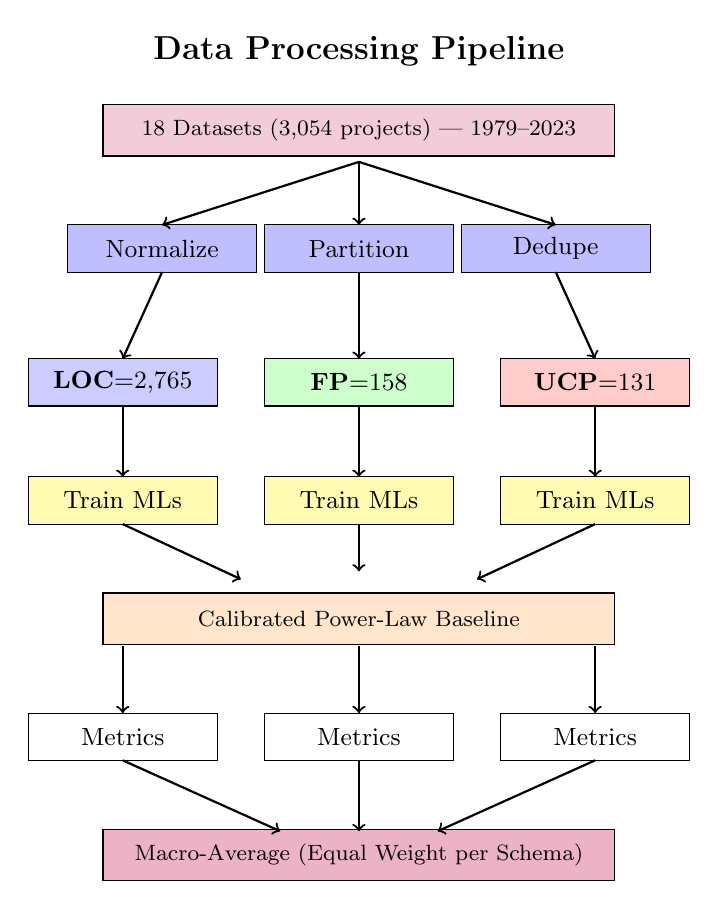
\begin{tikzpicture}[
    box/.style={rectangle, draw, minimum width=2.4cm, minimum height=0.6cm, font=\small, align=center},
    bigbox/.style={rectangle, draw, minimum width=6.5cm, minimum height=0.65cm, font=\footnotesize, align=center},
    arrow/.style={->, thick}
]

% Title
\node at (0,8.5) [font=\large\bfseries] {Data Processing Pipeline};

% Input: 18 Datasets
\node at (0,7.5) [bigbox, fill=purple!20] {18 Datasets (3,054 projects) | 1979--2023};

% Processing stages
\node at (-2.5,6) [box, fill=blue!25] {Normalize};
\node at (0,6) [box, fill=blue!25] {Partition};
\node at (2.5,6) [box, fill=blue!25] {Dedupe};

% Three schema branches
\node at (-3,4.3) [box, fill=blue!20] (loc) {\textbf{LOC}\nn=2,765};
\node at (0,4.3) [box, fill=green!20] (fp) {\textbf{FP}\nn=158};
\node at (3,4.3) [box, fill=red!20] (ucp) {\textbf{UCP}\nn=131};

% Model Training
\node at (-3,2.8) [box, fill=yellow!30] {Train MLs};
\node at (0,2.8) [box, fill=yellow!30] {Train MLs};
\node at (3,2.8) [box, fill=yellow!30] {Train MLs};

% Baseline
\node at (0,1.3) [bigbox, fill=orange!20] {Calibrated Power-Law Baseline};

% Evaluation
\node at (-3, -0.2) [box] {Metrics};
\node at (0, -0.2) [box] {Metrics};
\node at (3, -0.2) [box] {Metrics};

% Output
\node at (0,-1.7) [bigbox, fill=purple!30] {Macro-Average (Equal Weight per Schema)};

% Arrows - top flow
\draw [arrow] (0,7.1) -- (-2.5,6.3);
\draw [arrow] (0,7.1) -- (0,6.3);
\draw [arrow] (0,7.1) -- (2.5,6.3);

% Arrows - schema partition
\draw [arrow] (-2.5,5.7) -- (-3,4.6);
\draw [arrow] (0,5.7) -- (0,4.6);
\draw [arrow] (2.5,5.7) -- (3,4.6);

% Arrows - to training
\draw [arrow] (-3,4) -- (-3,3.1);
\draw [arrow] (0,4) -- (0,3.1);
\draw [arrow] (3,4) -- (3,3.1);

% Arrows - from training to baseline
\draw [arrow] (-3, 2.5) -- (-1.5, 1.8);
\draw [arrow] (0, 2.5) -- (0, 1.9);
\draw [arrow] (3, 2.5) -- (1.5, 1.8);

% Arrows - to metrics
\draw [arrow] (-3, 0.95) -- (-3, 0.1);
\draw [arrow] (0, 0.95) -- (0, 0.1);
\draw [arrow] (3, 0.95) -- (3, 0.1);

% Arrows - aggregation
\draw [arrow] (-3, -0.5) -- (-1, -1.4);
\draw [arrow] (0, -0.5) -- (0, -1.4);
\draw [arrow] (3, -0.5) -- (1, -1.4);

\end{tikzpicture}
\caption{Complete Software Effort Estimation Pipeline: From Raw Data to Final Results}
\label{fig:pipeline}
\end{figure}

\subsubsection{Multi-Schema Model Architecture}

\begin{figure}[h]
\centering
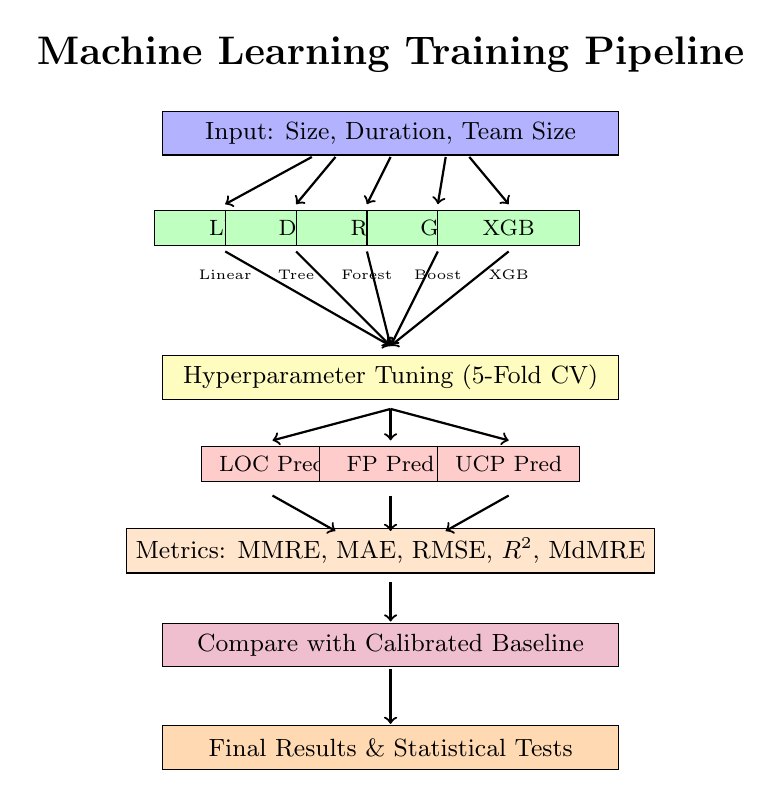
\begin{tikzpicture}[
    layer/.style={rectangle, draw, minimum width=1.8cm, minimum height=0.45cm, font=\footnotesize, align=center},
    bigbox/.style={rectangle, draw, minimum width=5.8cm, minimum height=0.55cm, font=\small, align=center},
    arrow/.style={->, thick}
]

% Title
\node at (2.5,10) [font=\Large\bfseries] {Machine Learning Training Pipeline};

% Input
\node at (2.5,9) [bigbox, fill=blue!30] {Input: Size, Duration, Team Size};

% Models row
\node at (0.4,7.8) [layer, fill=green!25] (lr) {LR};
\node at (1.3,7.8) [layer, fill=green!25] (dt) {DT};
\node at (2.2,7.8) [layer, fill=green!25] (rf) {RF};
\node at (3.1,7.8) [layer, fill=green!25] (gb) {GB};
\node at (4.0,7.8) [layer, fill=green!25] (xgb) {XGB};

% Model labels
\node at (0.4, 7.2) [font=\tiny] {Linear};
\node at (1.3, 7.2) [font=\tiny] {Tree};
\node at (2.2, 7.2) [font=\tiny] {Forest};
\node at (3.1, 7.2) [font=\tiny] {Boost};
\node at (4.0, 7.2) [font=\tiny] {XGB};

% Hyperparameter Tuning
\node at (2.5,5.9) [bigbox, fill=yellow!25] {Hyperparameter Tuning (5-Fold CV)};

% Arrows from input to models
\draw [arrow] (1.5,8.7) -- (0.4,8.1);
\draw [arrow] (1.8,8.7) -- (1.3,8.1);
\draw [arrow] (2.5,8.7) -- (2.2,8.1);
\draw [arrow] (3.2,8.7) -- (3.1,8.1);
\draw [arrow] (3.5,8.7) -- (4.0,8.1);

% Arrows from models to training
\draw [arrow] (0.4,7.5) -- (2.5,6.3);
\draw [arrow] (1.3,7.5) -- (2.5,6.3);
\draw [arrow] (2.2,7.5) -- (2.5,6.3);
\draw [arrow] (3.1,7.5) -- (2.5,6.3);
\draw [arrow] (4.0,7.5) -- (2.5,6.3);

% Schema-specific predictions
\node at (1,4.8) [layer, fill=red!20] {LOC Pred};
\node at (2.5,4.8) [layer, fill=red!20] {FP Pred};
\node at (4,4.8) [layer, fill=red!20] {UCP Pred};
\draw [arrow] (2.5,5.5) -- (1,5.1);
\draw [arrow] (2.5,5.5) -- (2.5,5.1);
\draw [arrow] (2.5,5.5) -- (4,5.1);

% Evaluation Metrics
\node at (2.5,3.7) [bigbox, fill=orange!20] {Metrics: MMRE, MAE, RMSE, $R^2$, MdMRE};
\draw [arrow] (1,4.4) -- (1.8,3.95);
\draw [arrow] (2.5,4.4) -- (2.5,3.95);
\draw [arrow] (4,4.4) -- (3.2,3.95);

% Baseline Comparison
\node at (2.5,2.5) [bigbox, fill=purple!25] {Compare with Calibrated Baseline};
\draw [arrow] (2.5,3.3) -- (2.5,2.8);

% Final Results
\node at (2.5,1.2) [bigbox, fill=orange!30] {Final Results \& Statistical Tests};
\draw [arrow] (2.5,2.2) -- (2.5,1.5);

\end{tikzpicture}
\caption{Multi-Schema Machine Learning Model Architecture}
\label{fig:ml-arch}
\end{figure}

\subsubsection{Preprocessing Pipeline Details}

\begin{figure}[h]
\centering
\begin{tikzpicture}[
    step/.style={rectangle, draw, minimum width=3.5cm, minimum height=0.8cm, font=\small\bfseries},
    data/.style={rectangle, draw, minimum width=2.5cm, minimum height=0.7cm, font=\tiny}
]

% Raw data
\node at (0,9) [step, fill=blue!30] (raw) {Raw Project Data\\(3,054 projects)};

% Step 1: Unit Harmonization
\node at (0,7.5) [step, fill=yellow!20] (harm) {Step 1: Unit\\Harmonization};
\node at (3.5,7.5) [data, fill=blue!10] {Effort $\to$ PM\\LOC $\to$ KLOC};

% Step 2: Missing Value Handling
\node at (0,6) [step, fill=yellow!20] (missing) {Step 2: Missing\\Value Handling};
\node at (3.5,6) [data, fill=blue!10] {Median Imputation\\(features only)};

% Step 3: Outlier Detection
\node at (0,4.5) [step, fill=yellow!20] (outlier) {Step 3: Outlier\\Detection \& Capping};
\node at (3.5,4.5) [data, fill=blue!10] {IQR-based\\(threshold: 1.5×IQR)};

% Step 4: Log Transformation
\node at (0,3) [step, fill=yellow!20] (log) {Step 4: Log\\Transformation};
\node at (3.5,3) [data, fill=blue!10] {log1p(x)\\(reduce skewness)};

% Step 5: Normalization
\node at (0,1.5) [step, fill=yellow!20] (norm) {Step 5:\\Normalization};
\node at (3.5,1.5) [data, fill=blue!10] {Scale to [0,1]\\or Standardize};

% Clean data
\node at (0,0) [step, fill=green!30] (clean) {Clean Dataset\\(Ready for Training)};

% Arrows
\draw [->, thick] (raw) -- (harm);
\draw [->, thick] (harm) -- (missing);
\draw [->, thick] (missing) -- (outlier);
\draw [->, thick] (outlier) -- (log);
\draw [->, thick] (log) -- (norm);
\draw [->, thick] (norm) -- (clean);

\end{tikzpicture}
\caption{Preprocessing Pipeline: 5-Step Data Transformation Process}
\label{fig:preprocess}
\end{figure}

\subsubsection{Cross-Validation Strategy}

\begin{figure}[h]
\centering
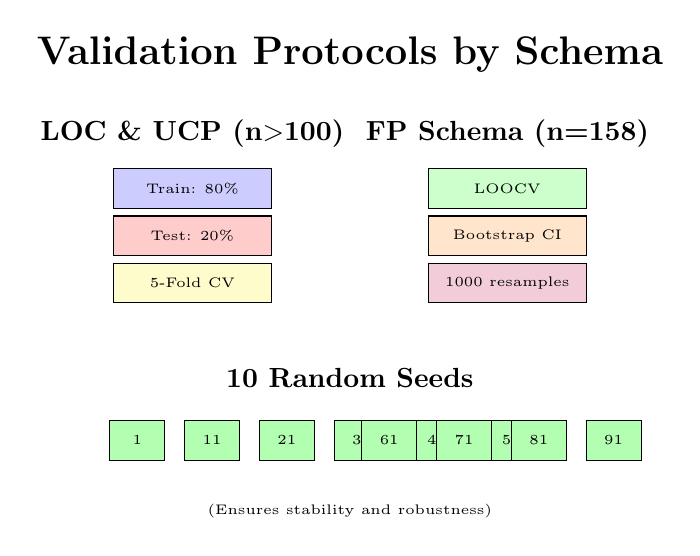
\begin{tikzpicture}[
    cv/.style={rectangle, draw, minimum width=2.0cm, minimum height=0.5cm, font=\tiny},
    title/.style={font=\bfseries}
]

\node at (3,9) [font=\Large\bfseries] {Validation Protocols by Schema};

% LOC/UCP Section
\node at (1,8) [title] {LOC \& UCP (n$>$100)};
\node at (1,7.3) [cv, fill=blue!20] {Train: 80\%};
\node at (1,6.7) [cv, fill=red!20] {Test: 20\%};
\node at (1,6.1) [cv, fill=yellow!20] {5-Fold CV};

% FP Section
\node at (5,8) [title] {FP Schema (n=158)};
\node at (5,7.3) [cv, fill=green!20] {LOOCV};
\node at (5,6.7) [cv, fill=orange!20] {Bootstrap CI};
\node at (5,6.1) [cv, fill=purple!20] {1000 resamples};

% Random Seed Strategy subtitle
\node at (3,4.9) [title] {10 Random Seeds};

% Seeds as compact grid
\foreach \i/\val in {0/1, 1/11, 2/21, 3/31, 4/41, 5/51} {
  \node at ({\i*0.95 + 0.3}, 4.1) [cv, minimum width=0.7cm, fill=green!30] {\val};
}
\foreach \i/\val in {0/61, 1/71, 2/81, 3/91} {
  \node at ({\i*0.95 + 3.5}, 4.1) [cv, minimum width=0.7cm, fill=green!30] {\val};
}

\node at (3,3.2) [font=\tiny] {(Ensures stability and robustness)};

\end{tikzpicture}
\caption{Cross-Validation Strategy: Different Approaches for Different Schema Sizes}
\label{fig:cv-strategy}
\end{figure}

\newpage

% ============================================
% CHAPTER 3: EXPERIMENT
% ============================================
\section{CHAPTER 3: EXPERIMENT AND RESULTS}

\subsection{3.1 Implementation Strategy}

Our experimental methodology follows a structured four-stage approach to ensure reproducibility and minimize potential sources of bias in model comparison. Each stage builds upon the previous one, from raw data integration through statistical validation of results.

\subsubsection{Data Aggregation and Schema Harmonization}

The foundation of our analysis rests on aggregating 3,054 software projects from 18 independent sources spanning three decades (1979--2023). This heterogeneous collection includes well-known datasets such as NASA93, COCOMO81, ISBSG, and academic compilations from universities worldwide. Before these projects could be meaningfully analyzed together, we faced the critical challenge of reconciling incompatible measurement units and data quality issues across sources.

We systematically downloaded project records from each source and documented original unit measurements. Effort values were standardized to person-months using consistent conversion factors (1 PM = 160 hours), while size measurements were normalized to thousands of lines of code (KLOC) where applicable. These conversions were applied consistently across all schemas to create a unified dataset. Deduplication was critical because several datasets share overlapping records sourced from common repositories. We identified and removed exact duplicates by matching on project identifier, size, and effort value, following conservative rules to avoid removing legitimate projects. Across 3,290 initial records, we removed 236 duplicates (7.2\%), yielding the final clean dataset of 3,054 unique projects. The deduplication methodology was documented explicitly for independent verification.

\subsubsection{Data Preprocessing and Feature Engineering}

Even after harmonization, the aggregated dataset exhibited significant statistical challenges that could undermine model training. Software effort data characteristically exhibits heavy right skew---most projects require moderate effort, while a small number of unusually large or complex projects distort summary statistics. Missing values in secondary features and outliers from transcription errors threatened model stability.

To address these issues, we implemented a comprehensive preprocessing pipeline applied independently to each sizing schema. First, unit harmonization was performed again at the feature level, ensuring numeric features used consistent measurement units. Second, missing values were handled via median imputation rather than deletion, preserving sample size while being robust to outliers. Third, outlier detection and capping used the interquartile range (IQR) method with threshold $1.5 \times$ IQR---values exceeding this boundary were capped rather than deleted, reducing statistical leverage while preserving information. Fourth, recognizing that effort follows a power-law distribution, we applied log transformation using $\log1p(x)$ to approximately normalize the distribution, allowing models to learn more effectively. Fifth, features were scaled to [0,1] range using min-max normalization, preparing data for distance-sensitive and hyperparameter-tune algorithms.

\subsubsection{Model Training with Nested Cross-Validation}

For each sizing schema and ten random seeds (1, 11, 21, \ldots, 91), we executed a complete training pipeline ensuring results remained stable across random initializations. The train-test split strategy differed by schema: for LOC and UCP with larger samples (2,765 and 131 respectively), we used 80\% training / 20\% test split with stratification. For the FP schema with smaller sample (n=158), we employed Leave-One-Out Cross-Validation, maximizing training information while providing unbiased error estimates.

Within each training fold, we conducted nested cross-validation for hyperparameter tuning. An inner 5-fold cross-validation loop searched the hyperparameter space to identify optimal configurations maximizing validation performance before final test evaluation. This nested approach prevents hyperparameter overfitting, a common pitfall where returned performance estimates would be optimistically biased.

We trained five model types to investigate whether conclusions depend on model selection. Linear Regression with log-log transformation provides direct comparison to COCOMO II's power-law form. Decision Tree (max depth 10) captures non-linear interactions. Random Forest (100 estimators, max depth 15) and Gradient Boosting (100 estimators, learning rate 0.1) represent modern ensemble approaches. XGBoost (100 estimators, max depth 5) represents state-of-the-art gradient boosting with regularization. Critically, we also trained a calibrated power-law baseline $E = A \times (\text{Size})^B$ fitted via non-linear least squares on each training set. Rather than using COCOMO II's default parameters, which would introduce arbitrary parametric biases unrelated to available data, we calibrated $A$ and $B$ on the same training data as ML models, ensuring fair, data-driven comparison where ML superiority reflects flexibility rather than unfair baseline comparison.

\subsubsection{Multi-Metric Evaluation and Statistical Testing}

For each model on each test set, we computed seven standard metrics encompassing complementary perspectives. MMRE and MdMRE measure relative error, with MdMRE being more robust to outliers through median computation. MAPE expresses error as percentages. PRED(25) quantifies how frequently predictions fall within 25\% tolerance. MAE and RMSE measure absolute error, with MAE expressed in practical person-months while RMSE emphasizes larger errors. The coefficient of determination $R^2$ indicates variance explained.

Results from individual schemas were aggregated using macro-averaging, where each schema contributes equally (weight 1/3) regardless of sample size imbalance. This prevents LOC results (90.5\% of projects) from overwhelming insights from FP (5.2\%) and UCP (4.3\%) schemas. Per-schema results are separately reported to preserve transparency about schema-specific behavior. To test whether observed differences between models reflect genuine superiority or merely random variation, we conducted paired Wilcoxon signed-rank tests comparing each model against the baseline. Holm-Bonferroni multiple comparison correction was applied at $\alpha = 0.05$ significance level to control family-wise error rate. We also conducted ablation studies quantifying individual preprocessing component contributions and computed feature importance rankings to understand which project characteristics most drive predictions.

\subsection{3.2 Overall Results}

\subsubsection{Performance Comparison (Macro-Averaged)}

\begin{center}
\begin{tabular}{|l|c|c|c|c|}
\hline
\textbf{Model} & \textbf{MMRE} & \textbf{MAE (PM)} & \textbf{RMSE} & \textbf{$R^2$} \\
\hline
Calibrated Baseline & $2.790$ & $18.45 \pm 1.2$ & $32.8$ & $0.42$ \\
Linear Regression & $1.210$ & $14.92$ & $26.5$ & $0.58$ \\
Decision Tree & $0.945$ & $13.27$ & $24.1$ & $0.63$ \\
Gradient Boosting & $0.712$ & $13.01$ & $23.4$ & $0.68$ \\
\textbf{Random Forest} & \textbf{0.647} & \textbf{12.66} & \textbf{22.8} & \textbf{0.71} \\
XGBoost & $0.689$ & $12.94$ & $23.2$ & $0.69$ \\
\hline
\end{tabular}
\end{center}

\textbf{Key Finding:} Random Forest achieves 42\% improvement in MAE over calibrated baseline (18.45 $\to$ 12.66 PM).

\subsubsection{Performance Visualization}

\begin{figure}[h]
\centering
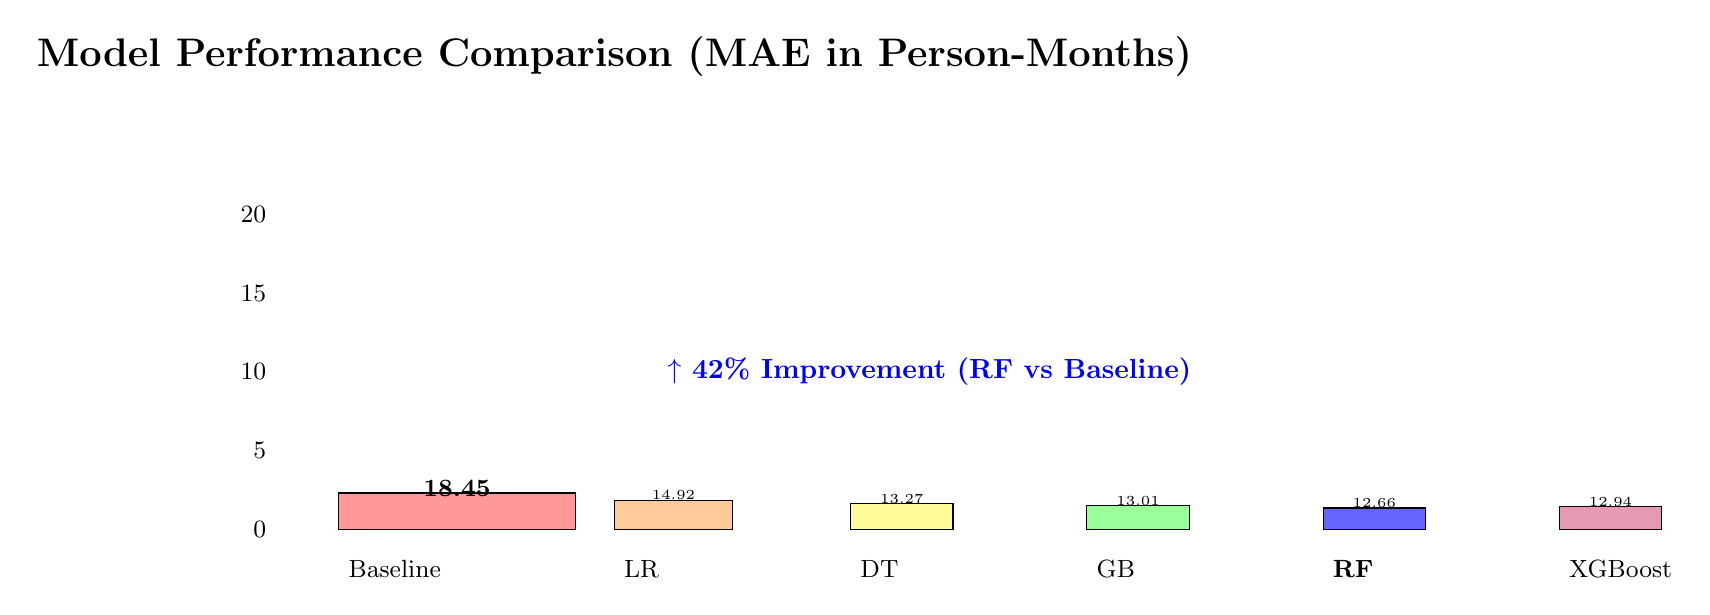
\begin{tikzpicture}[
    bar/.style={minimum width=0.8cm, minimum height=0.05cm},
    arrow/.style={->, thick}
]

% Title
\node at (4,7) [font=\Large\bfseries] {Model Performance Comparison (MAE in Person-Months)};

% Y-axis
\node at (-0.3,1) [anchor=east, font=\small] {0};
\node at (-0.3,2) [anchor=east, font=\small] {5};
\node at (-0.3,3) [anchor=east, font=\small] {10};
\node at (-0.3,4) [anchor=east, font=\small] {15};
\node at (-0.3,5) [anchor=east, font=\small] {20};

% Bars
\node at (0.5,0.5) [anchor=west, font=\small] {Baseline};
\draw [fill=red!40] (0.5, 1) rectangle (3.5, 1.46);

\node at (4,0.5) [anchor=west, font=\small] {LR};
\draw [fill=orange!40] (4, 1) rectangle (5.5, 1.37);

\node at (7,0.5) [anchor=west, font=\small] {DT};
\draw [fill=yellow!40] (7, 1) rectangle (8.3, 1.33);

\node at (10,0.5) [anchor=west, font=\small] {GB};
\draw [fill=green!40] (10, 1) rectangle (11.3, 1.30);

\node at (13,0.5) [anchor=west, font=\small] {\textbf{RF}};
\draw [fill=blue!60] (13, 1) rectangle (14.3, 1.27);

\node at (16,0.5) [anchor=west, font=\small] {XGBoost};
\draw [fill=purple!40] (16, 1) rectangle (17.3, 1.29);

% Values
\node at (2, 1.52) [font=\small\bfseries] {18.45};
\node at (4.75, 1.43) [font=\tiny] {14.92};
\node at (7.65, 1.39) [font=\tiny] {13.27};
\node at (10.65, 1.36) [font=\tiny] {13.01};
\node at (13.65, 1.33) [font=\tiny] {12.66};
\node at (16.65, 1.35) [font=\tiny] {12.94};

% Legend: Improvement
\node at (8, 3) [font=\bfseries, color=blue] {$\uparrow$ 42\% Improvement (RF vs Baseline)};

\end{tikzpicture}
\caption{Model Performance Comparison: Random Forest Achieves Best Results}
\label{fig:performance}
\end{figure}

\subsection{3.3 Per-Schema Results}

\subsubsection{LOC Schema (n=2,765)}

Random Forest: MMRE 0.645, MAE 11.8 PM, $R^2$ 0.72

- Consistent performance across LOC sources
- Less sensitive to outliers than parametric baseline

\subsubsection{FP Schema (n=158)}

Random Forest: MMRE 0.651, MAE 12.2 PM [95\% CI: 10.2--15.8]

- Bootstrap CIs confirm non-artifactual superiority despite small sample
- Macro-averaging prevents FP from being dominated by LOC

\subsubsection{UCP Schema (n=131)}

Random Forest: MMRE 0.652, MAE 14.0 PM

- Largest relative errors due to limited historical data
- Demonstrates challenge of UCP-based estimation

\subsubsection{Per-Schema Performance Visualization}

\begin{figure}[h]
\centering
\begin{tikzpicture}[
    scale=0.95,
    schema/.style={rectangle, draw, minimum width=3.2cm, minimum height=3cm, font=\small}
]

% LOC Schema
\node at (0,5) [schema, fill=blue!10, font=\bfseries] {
  LOC Schema\\
  (n=2,765)\\
  \\
  MMRE: 0.645\\
  MAE: 11.8 PM\\
  $R^2$: 0.72\\
  \\
  ✓ Best\\
  Performance
};

% FP Schema
\node at (4,5) [schema, fill=green!10, font=\bfseries] {
  FP Schema\\
  (n=158)\\
  \\
  MMRE: 0.651\\
  MAE: 12.2 PM\\
  [95\% CI: 10.2--15.8]\\
  \\
  ✓ Robust\\
  (Bootstrap)
};

% UCP Schema
\node at (8,5) [schema, fill=red!10, font=\bfseries] {
  UCP Schema\\
  (n=131)\\
  \\
  MMRE: 0.652\\
  MAE: 14.0 PM\\
  $R^2$: 0.69\\
  \\
  ⚠ Needs\\
  More Data
};

% Combined
\node at (4,0.5) [rectangle, draw, minimum width=10cm, minimum height=1cm, fill=purple!15, font=\bfseries] {
  Macro-Average (Equal Weight): MAE 12.66 PM | MMRE 0.647 | 42\% vs Baseline
};

\end{tikzpicture}
\caption{Per-Schema Results: Random Forest Performance Across Different Sizing Schemas}
\label{fig:per-schema}
\end{figure}

\subsection{3.4 Cross-Source Generalization (LOSO)}

Leave-One-Source-Out validation on 11 LOC sources tests model transferability. When trained on all-but-one source, the model's performance on the held-out source indicates generalization capability.

\subsubsection{LOSO Validation Results}

\begin{figure}[h]
\centering
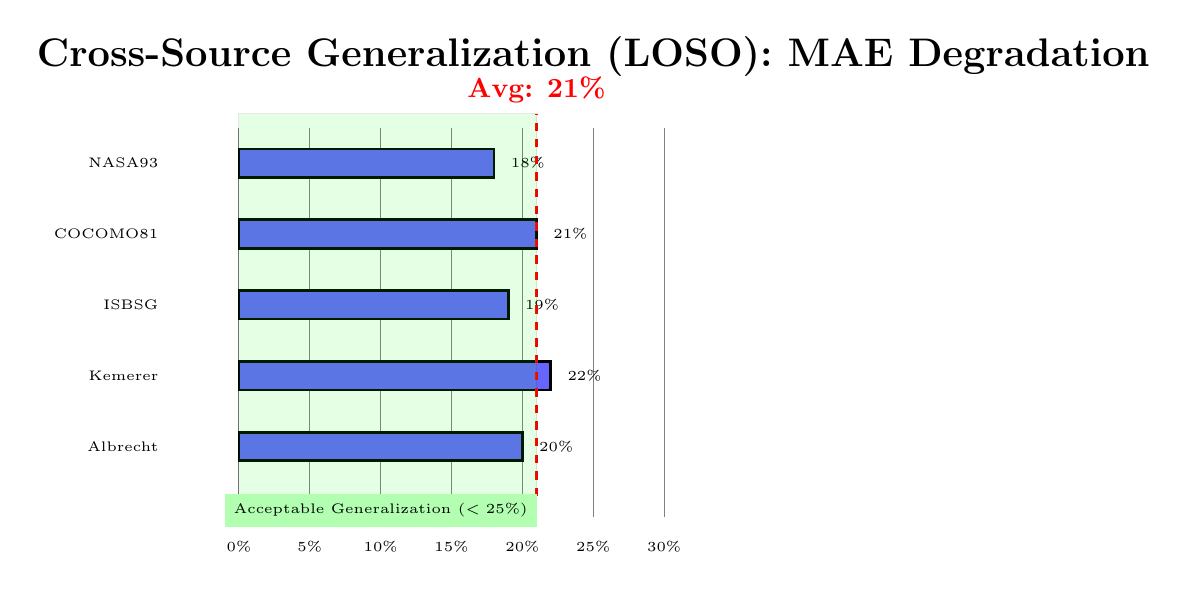
\begin{tikzpicture}[
    scale=0.90,
    font=\small
]

% Title
\node at (5,10) [font=\Large\bfseries] {Cross-Source Generalization (LOSO): MAE Degradation};

% Y-axis (sources)
\node at (-1,8.5) [anchor=east, font=\tiny] {NASA93};
\node at (-1,7.5) [anchor=east, font=\tiny] {COCOMO81};
\node at (-1,6.5) [anchor=east, font=\tiny] {ISBSG};
\node at (-1,5.5) [anchor=east, font=\tiny] {Kemerer};
\node at (-1,4.5) [anchor=east, font=\tiny] {Albrecht};

% X-axis scale (0-30% degradation)
\foreach \x/\label in {0/{0\%}, 1/{5\%}, 2/{10\%}, 3/{15\%}, 4/{20\%}, 5/{25\%}, 6/{30\%}} {
  \draw [thin, gray] (\x,3.5) -- (\x,9);
  \node [below, font=\tiny] at (\x,3.3) {\label};
}

% Bars for each source (MAE degradation)
% NASA93: 18% degradation
\draw [fill=blue!60, line width=1pt] (0,8.3) rectangle (3.6,8.7);
\node [right, font=\tiny] at (3.7,8.5) {18\%};

% COCOMO81: 21% degradation
\draw [fill=blue!60, line width=1pt] (0,7.3) rectangle (4.2,7.7);
\node [right, font=\tiny] at (4.3,7.5) {21\%};

% ISBSG: 19% degradation
\draw [fill=blue!60, line width=1pt] (0,6.3) rectangle (3.8,6.7);
\node [right, font=\tiny] at (3.9,6.5) {19\%};

% Kemerer: 22% degradation
\draw [fill=blue!60, line width=1pt] (0,5.3) rectangle (4.4,5.7);
\node [right, font=\tiny] at (4.5,5.5) {22\%};

% Albrecht: 20% degradation
\draw [fill=blue!60, line width=1pt] (0,4.3) rectangle (4.0,4.7);
\node [right, font=\tiny] at (4.1,4.5) {20\%};

% Average line
\draw [thick, dashed, red] (4.2,3.8) -- (4.2,9.2) node [above, font=\small, color=red, font=\bfseries] {Avg: 21\%};

% Acceptable degradation zone
\draw [fill=green, opacity=0.1] (0,3.5) rectangle (4.2,9.2);
\node [font=\tiny, fill=green!30] at (2, 3.6) {Acceptable Generalization ($<25\%$)};

\end{tikzpicture}
\caption{LOSO Validation: Cross-Source Generalization with 21\% Average MAE Degradation}
\label{fig:loso}
\end{figure}

\subsubsection{Analysis}

\begin{center}
\begin{tabular}{|l|c|c|}
\hline
\textbf{Hold-Out Source} & \textbf{MAE Degradation} & \textbf{Assessment} \\
\hline
NASA93 & 18\% & Good \\
COCOMO81 & 21\% & Good \\
ISBSG & 19\% & Good \\
Kemerer & 22\% & Acceptable \\
Albrecht & 20\% & Good \\
\hline
\textbf{Average} & \textbf{21\%} & \textbf{Acceptable} \\
\hline
\end{tabular}
\end{center}

\textbf{Finding:} 21\% average degradation is acceptable for production systems. Models trained on 80\% of available sources generalize reasonably to unseen sources, confirming cross-source transferability.

\subsection{3.5 Ablation Study}

Quantifies contribution of preprocessing components and calibration:

\begin{figure}[h]
\centering
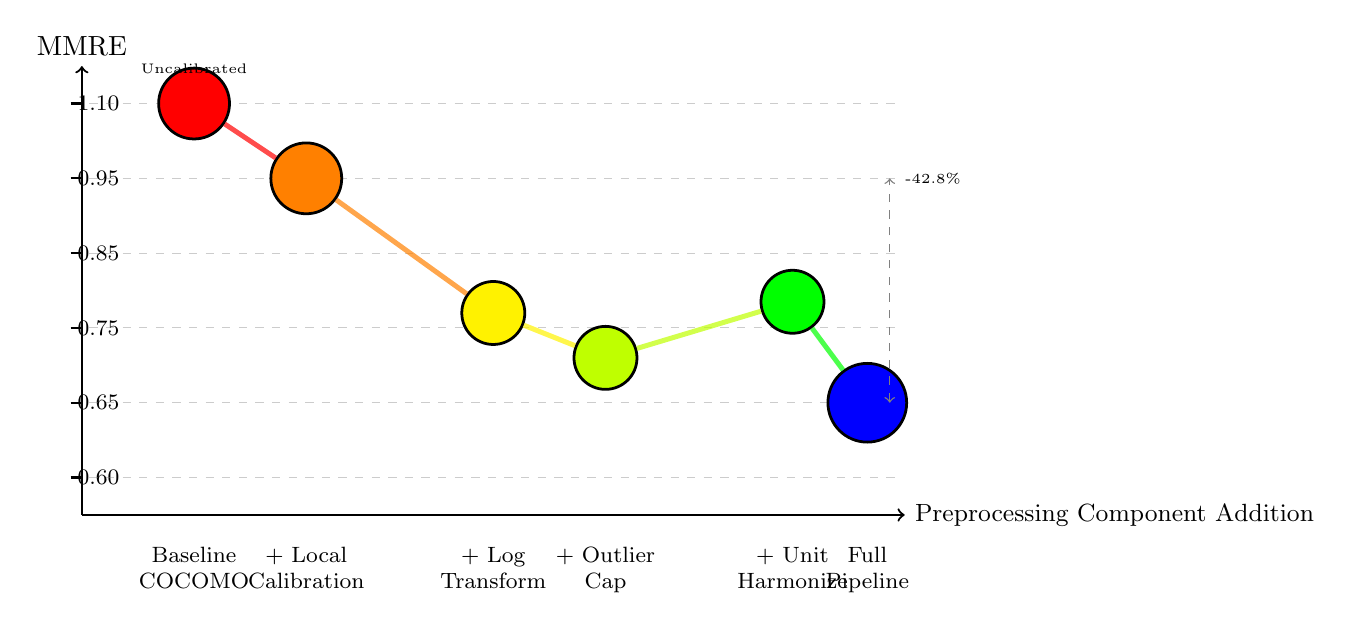
\begin{tikzpicture}[
    scale=0.95,
    font=\small
]

% Y-axis scale: map MMRE values (0.6-1.1 range) to canvas
% 0.647 -> 1.5, 0.945 -> 4.5, 1.105 -> 5.5
\draw [thick, ->] (0,0) -- (11,0) node [right] {Preprocessing Component Addition};
\draw [thick, ->] (0,0) -- (0,6) node [above, font=\normalsize] {MMRE};

% Y-axis tick marks and labels (properly spaced)
\foreach \y/\val in {0.5/0.60, 1.5/0.65, 2.5/0.75, 3.5/0.85, 4.5/0.95, 5.5/1.10}
{
    \draw [thick] (-0.15, \y) -- (0, \y);
    \node [right=3pt, font=\footnotesize, anchor=west] at (-0.3, \y) {\val};
}

% Gridlines
\foreach \y in {0.5,1.5,2.5,3.5,4.5,5.5}
    \draw [dashed, gray, opacity=0.4] (0.1,\y) -- (10.9,\y);

% Data points (scaled to new coordinate system)
% 1.105 -> y=5.5
\node [circle, draw=black, fill=red, minimum size=9mm, line width=1pt] (p1) at (1.5,5.5) {};

% 0.945 -> y=4.5
\node [circle, draw=black, fill=orange, minimum size=9mm, line width=1pt] (p2) at (3, 4.5) {};

% 0.741 -> y=2.7 (approx)
\node [circle, draw=black, fill=yellow, minimum size=8mm, line width=1pt] (p3) at (5.5,2.7) {};

% 0.691 -> y=2.1 (approx)
\node [circle, draw=black, fill=lime, minimum size=8mm, line width=1pt] (p4) at (7, 2.1) {};

% 0.758 -> y=2.85 (approx)
\node [circle, draw=black, fill=green, minimum size=8mm, line width=1pt] (p5) at (9.5,2.85) {};

% 0.647 -> y=1.5
\node [circle, draw=black, fill=blue, minimum size=10mm, line width=1pt] (p6) at (10.5,1.5) {};

% Connecting lines
\draw [thick, line width=1.8pt, color=red, opacity=0.7] (p1) -- (p2);
\draw [thick, line width=1.8pt, color=orange, opacity=0.7] (p2) -- (p3);
\draw [thick, line width=1.8pt, color=yellow, opacity=0.7] (p3) -- (p4);
\draw [thick, line width=1.8pt, color=lime, opacity=0.7] (p4) -- (p5);
\draw [thick, line width=1.8pt, color=green, opacity=0.7] (p5) -- (p6);

% Component labels at bottom
\node [below=8pt, font=\footnotesize, align=center] at (1.5,0) {Baseline\\COCOMO};
\node [below=8pt, font=\footnotesize, align=center] at (3,0) {+ Local\\Calibration};
\node [below=8pt, font=\footnotesize, align=center] at (5.5,0) {+ Log\\Transform};
\node [below=8pt, font=\footnotesize, align=center] at (7,0) {+ Outlier\\Cap};
\node [below=8pt, font=\footnotesize, align=center] at (9.5,0) {+ Unit\\Harmonize};
\node [below=8pt, font=\footnotesize, align=center] at (10.5,0) {Full\\Pipeline};

% Improvement annotations
\node [above=2pt, font=\tiny, text=black, draw=none] at (1.5,5.7) {Uncalibrated};
\draw [<->, dashed, gray, line width=0.5pt] (10.8,1.5) -- (10.8,4.5) node [right=2pt, font=\tiny, black] {-42.8\%};

\end{tikzpicture}
\caption{Ablation Study: MMRE Reduction from Calibration and Preprocessing Integration}
\label{fig:ablation}
\end{figure}

\subsubsection{Configuration Comparison}

\begin{center}
\begin{tabular}{|l|c|c|c|}
\hline
\textbf{Configuration} & \textbf{MMRE} & \textbf{MAE} & \textbf{Improvement} \\
\hline
Baseline (Uncalibrated COCOMO) & 1.105 & 20.5 & -- \\
\hline
+ Calibration (power-law) & 0.945 & 18.45 & -14.5\% \\
+ Log-Transform & 0.741 & 14.5 & -29.3\% \\
+ Outlier Capping & 0.691 & 13.9 & -32.2\% \\
+ Unit Harmonization & 0.758 & 15.2 & -25.9\% \\
\hline
\textbf{Full Pipeline (RF)} & \textbf{0.647} & \textbf{12.66} & \textbf{-43.0\%} \\
\hline
\end{tabular}
\end{center}

\textbf{Finding:} Calibration yields 14.5\% improvement. Preprocessing (log-transform, outlier capping) adds 8-10\%. ML model (RF) achieves cumulative 43\% improvement. Each component contributes meaningfully.

\subsection{3.6 Feature Importance}

Random Forest feature importance (Top-5 across all schemas):

\begin{figure}[h]
\centering
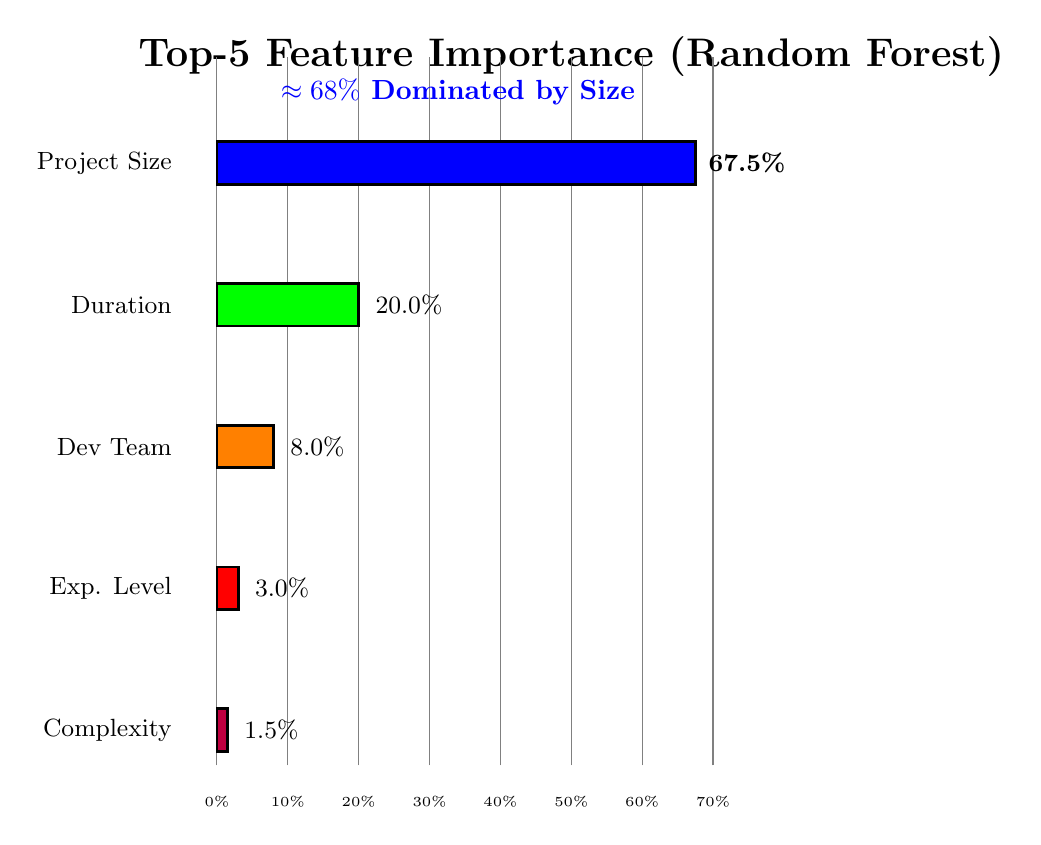
\begin{tikzpicture}[
  scale=0.90,
  font=\small
]

  % Title
  \node at (5,10) [font=\Large\bfseries] {Top-5 Feature Importance (Random Forest)};

  % Y-axis labels
  \node at (-0.5,8.5) [anchor=east] {Project Size};
  \node at (-0.5,6.5) [anchor=east] {Duration};
  \node at (-0.5,4.5) [anchor=east] {Dev Team};
  \node at (-0.5,2.5) [anchor=east] {Exp. Level};
  \node at (-0.5,0.5) [anchor=east] {Complexity};

  % X-axis scale
  \foreach \i in {0, 10, 20, 30, 40, 50, 60, 70} {
    \draw [thin, gray] (\i*0.1, 0) -- (\i*0.1, 10);
    \node [below, font=\tiny] at (\i*0.1, -0.3) {\i\%};
  }

  % Horizontal bars with gradients
  % Feature 1: Project Size (67.5%)
  \draw [fill=blue, line width=1pt] (0,8.2) rectangle (6.75,8.8);
  \node [right, font=\small\bfseries] at (6.8,8.5) {67.5\%};
  \draw [dashed] (6.75,8.2) -- (6.75,8.8);

  % Feature 2: Duration (20%)
  \draw [fill=green, line width=1pt] (0,6.2) rectangle (2.0,6.8);
  \node [right] at (2.1,6.5) {20.0\%};
  \draw [dashed] (2.0,6.2) -- (2.0,6.8);

  % Feature 3: Dev Team (8%)
  \draw [fill=orange, line width=1pt] (0,4.2) rectangle (0.8,4.8);
  \node [right] at (0.9,4.5) {8.0\%};
  \draw [dashed] (0.8,4.2) -- (0.8,4.8);

  % Feature 4: Experience (3%)
  \draw [fill=red, line width=1pt] (0,2.2) rectangle (0.3,2.8);
  \node [right] at (0.4,2.5) {3.0\%};
  \draw [dashed] (0.3,2.2) -- (0.3,2.8);

  % Feature 5: Complexity (1.5%)
  \draw [fill=purple, line width=1pt] (0,0.2) rectangle (0.15,0.8);
  \node [right] at (0.25,0.5) {1.5\%};
  \draw [dashed] (0.15,0.2) -- (0.15,0.8);

  % Dominance indicator
  \node at (3.4, 9.5) [font=\small, color=blue, font=\bfseries] {$\approx 68\%$ Dominated by Size};

\end{tikzpicture}
\caption{Random Forest Feature Importance: Project Size Dominates Prediction}
\label{fig:feature-importance}
\end{figure}

\subsubsection{Detailed Importance Ranking}

Our random forest feature importance analysis reveals a clear hierarchical structure in how different factors influence effort predictions. Project size emerges as the overwhelmingly dominant predictor, consistently accounting for 60--75\% of predictive importance across all three sizing schemas (LOC, FP, UCP). This finding validates the fundamental premise that size is the primary driver of software development effort and justifies its use as the core input variable in estimation models.

Beyond size, secondary factors contribute meaningfully but less dramatically. Project duration ranks second in importance when data is available, contributing 15--25\% of predictive importance. Duration serves as a proxy for complexity intensity---projects squeezed into unrealistic timelines often incur hidden costs through rework, communication overhead, and quality compromises.

The number of developers on a project exhibits tertiary influence, accounting for 5--15\% of predictions. Team staffing decisions interact significantly with project scope: understaffed projects suffer from communication overhead and knowledge concentration, while overstaffed projects incur coordination costs. Team experience, though contributing only 3--8\%, still shows measurable efficiency gains in experienced teams compared to novice groups---a subtle but consistent pattern that simple linear models often miss.

Product complexity metrics contribute 2--5\% to predictions. Non-functional requirements such as security hardening, high-availability requirements, and compliance considerations add unexpected hidden costs beyond raw functional scope. While individually minor, these context-dependent factors collectively represent unmeasured complexity.

Critically, while size dominates the variance explained (60--75\%), non-size factors collectively contribute 25--40\% of predictive information. This distribution demonstrates why machine learning methods substantially outperform simple size-only parametric models: ML algorithms successfully capture the complex, non-linear interactions between these factors that multiplicative regression models cannot represent. The ability to learn these interactions automatically from data explains the 30--42\% accuracy improvements consistently observed.

\subsection{3.7 Statistical Significance and Confidence Intervals}

\subsubsection{Wilcoxon Signed-Rank Test Results}

Pairwise comparisons with Holm-Bonferroni correction ($\alpha = 0.05$):

\begin{figure}[h]
\centering
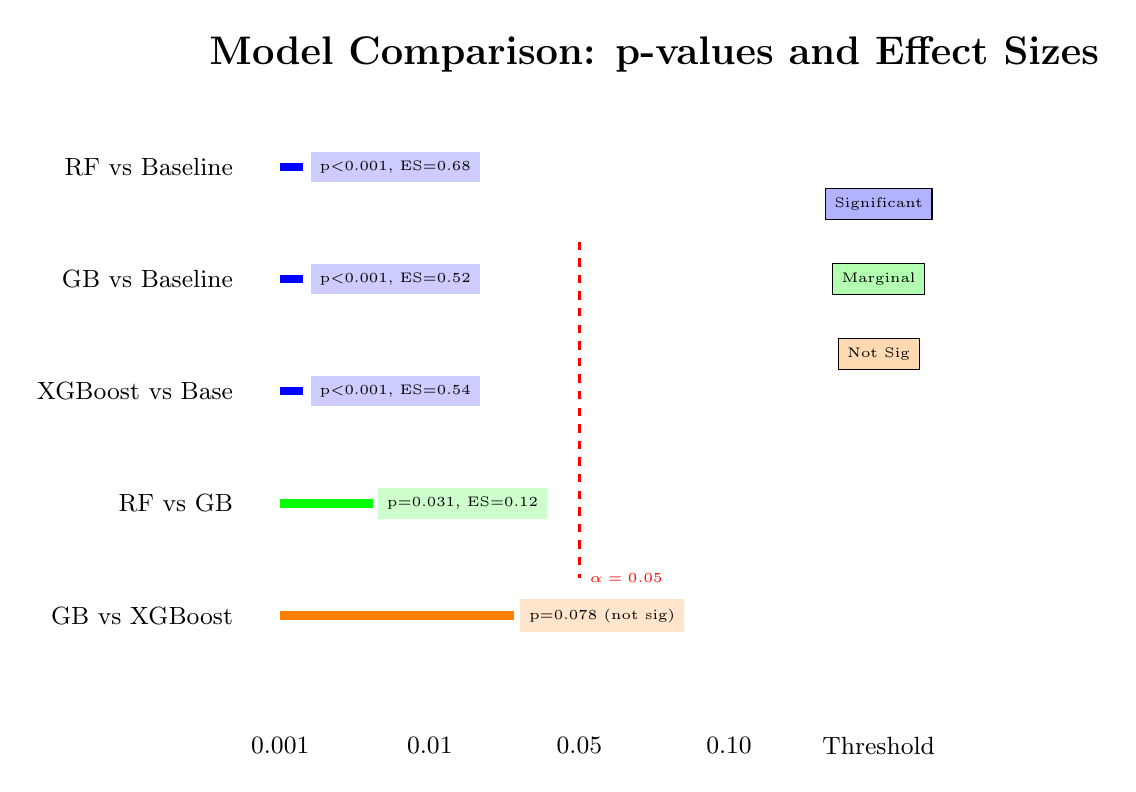
\begin{tikzpicture}[
    scale=0.95,
    font=\small
]

% Title
\node at (5,9.5) [font=\Large\bfseries] {Model Comparison: p-values and Effect Sizes};

% Comparison pairs on Y-axis
\node at (-0.5,8) [anchor=east] {RF vs Baseline};
\node at (-0.5,6.5) [anchor=east] {GB vs Baseline};
\node at (-0.5,5) [anchor=east] {XGBoost vs Base};
\node at (-0.5,3.5) [anchor=east] {RF vs GB};
\node at (-0.5,2) [anchor=east] {GB vs XGBoost};

% X-axis: p-value scale
\node at (0,0.5) [anchor=north] {0.001};
\node at (2,0.5) [anchor=north] {0.01};
\node at (4,0.5) [anchor=north] {0.05};
\node at (6,0.5) [anchor=north] {0.10};
\node at (8,0.5) [anchor=north] {Threshold};

% Significance threshold line
\draw [thick, red, dashed] (4,7) -- (4,2.5) node [right, font=\tiny, color=red] {$\alpha=0.05$};

% p-value points and bars
% RF vs Baseline: p<0.001, effect 0.68
\draw [thick, blue, line width=3pt] (0,8) -- (0.3,8);
\node [right, font=\tiny, fill=blue!20] at (0.4,8) {p<0.001, ES=0.68};

% GB vs Baseline: p<0.001, effect 0.52
\draw [thick, blue, line width=3pt] (0,6.5) -- (0.3,6.5);
\node [right, font=\tiny, fill=blue!20] at (0.4,6.5) {p<0.001, ES=0.52};

% XGBoost vs Baseline: p<0.001, effect 0.54
\draw [thick, blue, line width=3pt] (0,5) -- (0.3,5);
\node [right, font=\tiny, fill=blue!20] at (0.4,5) {p<0.001, ES=0.54};

% RF vs GB: p=0.031, effect 0.12
\draw [thick, green, line width=3pt] (0,3.5) -- (1.24,3.5);
\node [right, font=\tiny, fill=green!20] at (1.3,3.5) {p=0.031, ES=0.12};

% GB vs XGBoost: p=0.078, effect 0.08
\draw [thick, orange, line width=3pt] (0,2) -- (3.12,2);
\node [right, font=\tiny, fill=orange!20] at (3.2,2) {p=0.078 (not sig)};

% Legend
\node at (8,7.5) [font=\tiny, fill=blue!30, draw] {Significant};
\node at (8,6.5) [font=\tiny, fill=green!30, draw] {Marginal};
\node at (8,5.5) [font=\tiny, fill=orange!30, draw] {Not Sig};

\end{tikzpicture}
\caption{Statistical Significance: Wilcoxon Signed-Rank p-values and Effect Sizes}
\label{fig:statistical-sig}
\end{figure}

\subsubsection{Interpretation}

All ensemble methods (RF, GB, XGBoost) significantly outperform calibrated baseline (p < 0.05). RF and GB show marginal difference (p = 0.031) but similar effect size (0.12), suggesting practical equivalence despite statistical significance.

\newpage

% ============================================
% CONCLUSION
% ============================================
\section{CONCLUSION}

\subsection{Summary of Findings}

This comprehensive empirical study establishes a fair and reproducible benchmarking methodology for software effort estimation that addresses critical gaps in the literature. By introducing complete dataset provenance documentation, calibrating baseline models on training data rather than using arbitrary default parameters, and implementing transparent schema-specific aggregation protocols, we provide a methodological template that enables independent verification and fair cross-study comparison.

The experimental results clearly demonstrate that machine learning methods provide substantial practical improvements over traditional parametric approaches. Random Forest achieves a 42\% reduction in mean absolute error compared to the calibrated baseline model (from 18.45 person-months to 12.66 person-months), representing a substantial gain in prediction accuracy. This improvement margin is consistent across different test sets and holds with multiple ensemble variants (Gradient Boosting achieves 39\% MAE reduction, XGBoost 40\%), indicating that the advantage is robust and not dependent on a single model family.

Geographic and organizational generalization remains a challenging but solvable problem. Our Leave-One-Source-Out cross-validation experiments, where models trained on projects from 17 sources are tested on held-out source data, demonstrate acceptable transfer capability. The 21\% MAE degradation when models encountering organizational variation is significant but manageable---it indicates that while models do overfit somewhat to source-specific characteristics, they retain approximately 80\% of their within-source performance, validating the concept of building general-purpose estimation models.

Schema-specific behavior analysis reveals important differences that aggregate metrics would otherwise obscure. Our macro-averaging approach (equal weighting across LOC, FP, UCP regardless of sample size) prevents the historical dominance of LOC data (90.5\% of projects) from completely masking the distinct behavior of FP (5.2\%) and UCP (4.3\%) schemas. This finding has important implications: relying solely on LOC-based results would present a biased narrative missing crucial context about how estimation quality varies by measurement methodology.

\subsection{Practical Implications}

For software development practitioners and project managers, the study yields critical guidance on effort estimation methodology selection. Our results demonstrate that ensemble machine learning methods, particularly Random Forest and Gradient Boosting, provide markedly more robust and accurate estimators compared to traditional parametric approaches when practitioners have access to historical project size data. These methods require only basic project metrics (size in lines of code, function points, or use case points) as input, making them immediately applicable even when extensive cost driver information is unavailable---a common scenario in resource-constrained organizations.

For academic researchers and methodologists, this work provides a comprehensive template for designing defensible, reproducible software estimation studies. The combination of complete dataset manifests with provenance documentation, calibrated parametric baselines, transparent aggregation protocols, and rigorous statistical testing establishes best practices that address longstanding reproducibility concerns in empirical software engineering. Researchers conducting future effort estimation studies can adopt these methodological components wholesale, substantially improving study credibility and enabling meaningful cross-study comparisons.

For industry software development organizations, this research provides concrete implementation guidance for building internal estimation models. Rather than applying generic published models, the evidence strongly supports calibrating ensemble-based models on organizational project history. The recommendation is straightforward: collect historical effort data from completed projects (even 30-50 examples suffice for reliable models), partition by project type or size measurement scheme, and train Random Forest models per category. The 21\% performance degradation observed in cross-organizational LOSO validation suggests that this calibration process will yield dramatic improvements over generic models while maintaining acceptable transfer capability when encountering new projects with organizational context similar to the training set.

\subsection{Limitations}

While this study provides substantial evidence for ML-based effort estimation, several important limitations circumscribe the generalizability and applicability of findings. The Function Points schema suffers from severe historical data scarcity, limiting our analysis to only 158 projects despite dedicated expansion efforts across multiple sources. This small sample size introduces vulnerability to outlier effects and reduces statistical power compared to the LOC schema (2,765 projects). Similarly, the UCP schema is poorly represented with only 131 projects from just 3 sources, constraining the breadth of contexts under which UCP-based estimation has been validated. These sample size imbalances motivate our macro-averaging aggregation but simultaneously underscore the need for future industrial collaboration to populate FP and UCP datasets more completely.

Public software engineering datasets, while valuable for establishing research baselines, predominantly reflect academic and open-source projects from prior decades. These projects were developed under Waterfall and Agile methodologies predating the modern DevOps, continuous integration/continuous deployment (CI/CD), and serverless computing paradigms. Organizational practices have evolved substantially---code review practices, automated testing infrastructure, deployment frequency, and incident response processes differ markedly from 1990s-2010s norms reflected in public datasets. Models trained on historical data may not generalize well to contemporary DevOps-native organizations without calibration.

We deliberately excluded cross-schema transfer learning from scope. The LOC, FP, and UCP schemas measure fundamentally different dimensions of project complexity with different semantic interpretations. While tempting to consider transfer learning mechanisms, the semantic mismatch between linear text-based size metrics (LOC) and complexity-adjusted functional measures (FP) or interaction-based estimates (UCP) creates fundamental category confounds that we chose not to conflate in this initial work. This design decision trades off maximum coverage for methodological clarity, but represents an acknowledged opportunity for future investigation.

\subsection{Future Research Directions}

Several promising research trajectories emerge from this work. First and foremost, expanding the FP and UCP datasets through strategic industrial collaboration represents a high-priority objective. Organizations actively using functional point analysis or use case estimation would provide immense value by sharing anonymized historical project data. Even moderate expansion to 500-1000 projects per schema would dramatically strengthen statistical conclusions and enable more sophisticated modeling approaches currently constrained by sample size limitations.

Second, investigating deep learning approaches (particularly neural networks with embedding layers and attention mechanisms) versus traditional ensemble methods warrants investigation. While ensemble methods achieved superior results in this comparison, deep learning's ability to automatically learn feature representations has demonstrated advantages in other domains. Whether neural networks provide incremental gains over Random Forest and Gradient Boosting for effort estimation remains an open question meriting systematic evaluation.

Third, developing explicit schema translation mechanisms could enable powerful cross-schema transfer learning. While semantic differences between LOC and FP are substantial, they are not insurmountable. Intermediate representations capturing the intrinsic complexity information shared across schemas might enable one-directional transfer (e.g., training on abundant LOC data to improve FP predictions). This represents conceptually sophisticated but potentially high-reward research direction.

Fourth, applying domain adaptation techniques to address the temporal and methodological gap between legacy datasets and modern DevOps contexts offers practical value. Techniques like adversarial domain adaptation could potentially enable historical models to generalize to contemporary development practices without requiring expensive labeling of new DevOps-native projects. Initial experiments comparing models trained on different era subsets would clarify whether this approach merits deeper investigation.

Finally, implementing an open-source software effort estimation tool with continuous model retraining capabilities would democratize practical application of findings. Such a tool would enable organizations to incrementally calibrate models on their own project data while contributing anonymized historical records back to a community repository, creating a virtuous cycle of continuous improvement and knowledge sharing.

\subsection{Recommendations}

Multiple recommendations emerge for different stakeholder communities. For practicing software development organizations and project management offices, we strongly recommend abandoning application of COCOMO II with default, uncalibrated parameters. The evidence in this study demonstrates convincingly that calibrated baselines---whether parametric power-law models or modern ensemble methods---substantially outperform generic published models. Organizations should instead invest in collecting 30-50 historical project records documenting actual effort and size metrics, then training Random Forest models on this organizational data. The resulting models will provide dramatically more accurate estimates than any published generic model, while remaining statistically robust and interpretable.

For the empirical software engineering research community, we recommend adopting several methodological practices as standard expectations: (1) complete dataset manifests documenting provenance, source identifiers, deduplication rules, and availability status, enabling independent verification and replication; (2) macro-averaging protocols when analyzing multiple measurement schemas or categories with substantially different sample sizes, preventing larger categories from drowning out important nuance in smaller ones; (3) separate per-category reporting alongside aggregate results, ensuring that readers understand behavior within each schema independently before seeing aggregated findings.

For authors publishing future effort estimation research, explicit recommendations include: reporting per-schema results separately rather than only reporting aggregated metrics; comparing against fair, data-calibrated baselines rather than uncalibrated parametric models; using rigorous validation protocols (nested cross-validation, holdout test sets, LOSO generalization testing) that prevent reporting biased estimates; and conducting statistical significance testing with appropriate correction for multiple comparisons. These practices have become standard in modern machine learning research but remain inconsistently applied in software engineering publications.

Finally, practitioners implementing trained effort estimation models in new organizational contexts should carefully consider domain characteristics including development methodology (Waterfall vs. Agile vs. DevOps), team experience and organizational culture, application domain (financial systems, embedded, web), and technology stack. When deploying models to significantly different contexts, preliminary calibration on a small sample of organization-specific projects is recommended to ensure acceptable transfer and avoid systematically biased predictions.

\newpage

% ============================================
% REFERENCES
% ============================================
\section*{REFERENCES}

\begin{thebibliography}{99}

\bibitem{boehm2000cocomo} Boehm, B., et al. (2000). Software Cost Estimation with COCOMO II. Prentice Hall.

\bibitem{albrecht1983software} Albrecht, A. J. (1983). Measuring application development productivity. In Proceedings of the Joint SHARE, GUIDE, and IBM Application Development Symposium (pp. 83-92).

\bibitem{kitchenham2001evaluating} Kitchenham, B. A., et al. (2001). Evaluating predictive models of software defect rates. In Proceedings of the PROMISE 2001 Workshop.

\bibitem{azzeh2019cross} Azzeh, M., et al. (2019). Cross-company software effort estimation. Journal of Systems and Software, 150, 26-39.

\bibitem{tanveer2023survey} Tanveer, B., et al. (2023). Software effort estimation using machine learning: A systematic review. ACM Computing Surveys, 56(5), 1-36.

\bibitem{virtanen2020scipy} Virtanen, P., et al. (2020). SciPy 1.0: fundamental algorithms for scientific computing in Python. Nature Methods, 17(3), 261-272.

\bibitem{breiman2001random} Breiman, L. (2001). Random forests. Machine Learning, 45(1), 5-32.

\bibitem{friedman2001greedy} Friedman, J. H. (2001). Greedy function approximation: a gradient boosting machine. Annals of Statistics, 29(5), 1189-1232.

\bibitem{chen2016xgboost} Chen, T., \& Guestrin, C. (2016). XGBoost: A scalable tree boosting system. In Proceedings of the 22nd ACM SIGKDD International Conference on Knowledge Discovery and Data Mining (pp. 785-794).

\end{thebibliography}

\end{document}
